\labelchapter{classes}{Classes and inheritance}

The simple objects that we have seen so far provide abstraction, but they provide
little in the way of software re-use, which is one of the key benefits of object-oriented
programming.  What exactly is object-oriented programming?  Mitchell~\cite{Mit03} points out four
fundamental properties.

\begin{itemize}
\item

\emph{Abstraction}:
the details of the implementation are hidden in the object; the interface is just the set of
publically-accessible methods.

\item

\emph{Subtyping}:
if an object \hbox{\lstinline/a/} has all the functionality of an object \hbox{\lstinline/b/}, then we may
use \hbox{\lstinline/a/} in any context where \hbox{\lstinline/b/} is expected.

\item

\emph{Dynamic lookup}:
when a message is sent to an object, the method to be executed is determined by the implementation
of the object, not by some static property of the program.  In other words, different objects may
react to the same message in different ways.

\item

\emph{Inheritance}:
the definition of one kind of object can be re-used to produce a new kind of object.
\end{itemize}
%
We have seen a little about first three features; we now look at inheritance.  In OCaml, like
many other languages, inheritance arises from classes, where a \emph{class} is a \emph{template}
that describes how to build an object.  Inheritance is the ability to create new classes (and thus
new objects) from existing ones by adding, removing, and modifying methods and fields.

\section{Class basics}

\index{classes!definitions}
\index{objects!classes}
Let's begin by defining a class.  The simplest form of a class definition looks like the definition
of an object, but using the keyword \hbox{\lstinline/class/} instead of \hbox{\lstinline/let/}.  Classes are not
objects in OCaml, and a class definition is not an expression.  Every class definition must occur at
the top level.

\label{keyword:class}
\begin{ocaml}
# class poly =
  object
     val vertices = [|(46, 70); (54, 70); (60, 150); (40, 150)|]
     method draw = Graphics.fill_poly vertices
  end;;
@
\begin{topoutput}
class poly : object val vertices : (int * int) array method draw : unit end
\end{topoutput}
@
\end{ocaml}
%
\index{new@\lstinline/new/}
\index{classes!new}
\label{keyword:new}
To create an object from a class, the keyword \hbox{\lstinline/new/} is used with the name of the class.

\begin{center}
\begin{tabular}{cc}
\begin{minipage}[b]{3in}
\begin{ocamllistingx}
# let p = new poly;;
@
\begin{topoutput}
val p : poly = <obj>
\end{topoutput}
@
# p#draw;;
@
\begin{topoutput}
- : unit = ()
\end{topoutput}
@
\end{ocamllistingx}
\end{minipage}
&
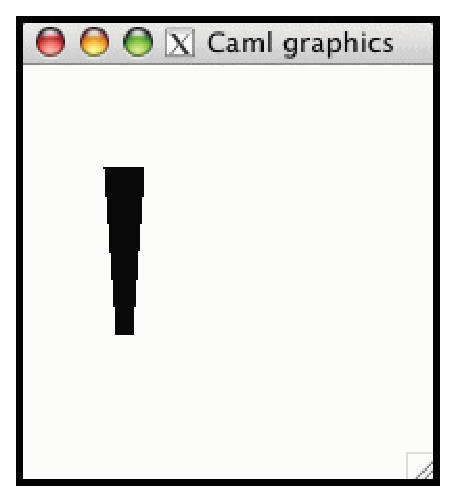
\includegraphics[scale=0.3]{graphics5}
\end{tabular}
\end{center}

\subsection{Class types}

There are a number of things happening here, so let's look at the parts.  First, we defined a
class called \hbox{\lstinline/poly/} with field \hbox{\lstinline/vertices/} and a method \hbox{\lstinline/draw/}.  The
class \hbox{\lstinline/poly/} has a \emph{class type} that specifies the type of its methods and fields.

\begin{ocaml}
object
   val vertices : (int * int) array
   method draw : unit
end
\end{ocaml}
%
\label{classes:types}
\index{class types}
Class types are something you may not have seen before, even if you are familiar with
object-oriented programming.  However, class types arise naturally in languages that include both
classes and modules.  In OCaml, every definition that can appear in a module must have a type.  A
class is not a type (because it contains code), so it must have a type.  Consider a module that
defines the blobs of the previous chapter.  The module \hbox{\lstinline/Blobs/} contains the class
definition, and the signature \hbox{\lstinline/BlobsSig/} declares the class and its type.

\begin{ocaml}
module Blobs : BlobsSig = struct         module type BlobsSig = sig
   class poly =                             class poly : 
   object                                   object
      val vertices = [||]                      val vertices : (int * int) array
      method draw =                            method draw : unit
         Graphics.fill_poly vertices        end
   end

   let p = new poly                         val p : poly
end;;                                    end;;
\end{ocaml}
%
Another thing to point out is that the polygon \hbox{\lstinline/p/} has type \hbox{\lstinline/val p : poly/}.
In this context, the class name \hbox{\lstinline/poly/} stands for the type of polygon
objects---that is, \hbox{\lstinline/type poly = < draw : unit >/}.  In general, whenever a class name appears in
the context of a type expression, it stands for an object type.  There is nothing special about the
class name.  Two classes that have methods with the same types stand for the same object type, as the
following example illustrates.

\index{gunfighter}
\begin{tabular}{l}
\begin{ocaml}
# class gunfighter =
  object
     method draw = print_string "Bang!\n"
  end;;
@
\begin{topoutput}
class gunfighter : object method draw : unit end
\end{topoutput}
@
# let p : gunfighter = new poly;;
@
\begin{topoutput}
val p : gunfighter = <obj>
\end{topoutput}
@
\end{ocaml}
\end{tabular}

\subsection{Parameterized classes}

\label{classes:parameterized}
\index{classes!constructors}
\index{classes!parameterized classes}
The current \hbox{\lstinline/poly/} class is not very useful because the vertices are fixed.  If we want
more than one polygon, we can define a \emph{parameterized class}.  A parameterized class definition
looks like a class definition that takes arguments; the arguments are passed to \hbox{\lstinline/new/} at
object creation time.

\begin{center}
\begin{tabular}{@{}cc}
\begin{minipage}[b]{3.5in}
\begin{ocamllistingx}
# class poly vertices =
  object
     val vertices = vertices
     method draw = Graphics.fill_poly vertices
  end;;
@
\begin{topoutput}
class poly : (int * int) array ->
  object val vertices : (int * int) array method draw : unit end
\end{topoutput}
@
# let p1 =
     new poly [|(46, 70); (54, 70); (60, 150); (40, 150)|];;
@
\begin{topoutput}
val p1 : poly = <obj>
\end{topoutput}
@
# let p2 = new poly [|(40, 40); (60, 40); (60, 60); (40, 60)|];;
@
\begin{topoutput}
val p2 : poly = <obj>
\end{topoutput}
@
# p1#draw; p2#draw;;
@
\begin{topoutput}
- : unit = ()
\end{topoutput}
@
\end{ocamllistingx}
\end{minipage}
&
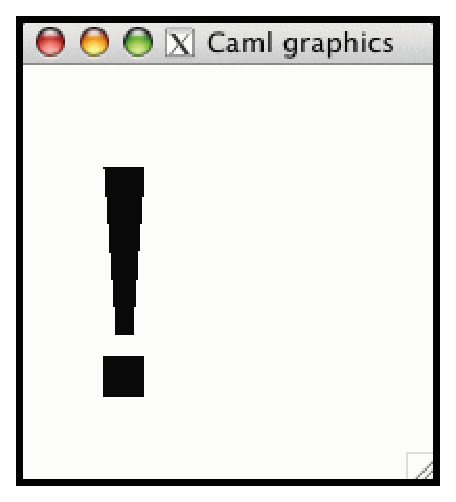
\includegraphics[scale=0.3]{graphics6}
\end{tabular}
\end{center}
%
In OCaml, there is no specific language feature called an object constructor.  Instead, the class
definition serves as its only constructor, and there is only one way to construct an object from a
class---by using \hbox{\lstinline/new/}.

In a class definition, any class expression can be used as the definition.  For example, the
following definition specifies that the class \hbox{\lstinline/rectangle/} is a specific kind
of \hbox{\lstinline/poly/}.

\begin{ocaml}
# class rectangle (x1, y1) (x2, x2) =
     poly [|(x1, y1); (x2, y1); (x2, y2); (x1, y2)|];;
@
\begin{topoutput}
class rectangle : float * float -> float * float -> poly
\end{topoutput}
@
\end{ocaml}

\subsection{Classes with let-expressions}

\label{classes:let}
\label{classes!let expressions}
Classes can be defined with leading let-definitions, which are evaluated before a new object is
created.  The let-definitions have the standard form.  For example, the following class defines a
regular polygon with \hbox{\lstinline/n/} sides.  The vertices of the polygon are computed before the
object is created.

\begin{ocaml}
class regular_poly n radius =
   let () = assert (n > 2) in
   let vertices = Array.create n (0, 0) in
   let step = 6.28 /. float_of_int n in
   let () =
      for i = 0 to n - 1 do
         let theta = float_of_int i *. step in
         let x = int_of_float (cos theta *. radius) in
         let y = int_of_float (sin theta *. radius) in
         vertices.(i) <- (x + 100, y + 100)
      done
   in
   object
      method draw = Graphics.fill_poly vertices
   end;;
\end{ocaml}
%
Syntactically, each leading expression must be a let-definition, so any computations that operate by
side-effect are written with a dummy let in the form \hbox{\lstinline/let () = $\cdots$ in/}.  The
assertion ensures that the polygon has at least 3 sides.

\begin{center}
\begin{tabular}{cc}
\begin{minipage}[b]{3in}
\begin{ocamllistingx}
# let p = new regular_poly 7 100.0;;
@
\begin{topoutput}
val p : regular_poly = <obj>
\end{topoutput}
@
# p#draw;;
@
\begin{topoutput}
- : unit = ()
\end{topoutput}
@
\end{ocamllistingx}
\end{minipage}
&
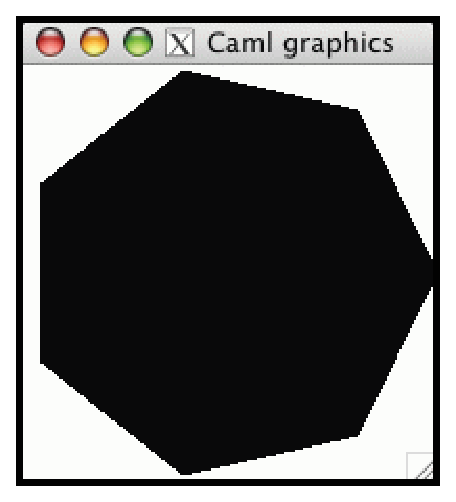
\includegraphics[scale=0.3]{regular-poly}
\end{tabular}
\end{center}

\subsection{Type inference}

\index{classes!type inference}
\index{classes!polymorphic}
If you have tried defining classes of your own, you may be running into a problem where OCaml is
inferring class types that are ``too polymorphic.''  Class types can be polymorphic, as we will see
in Chapter~\ref{chapter:polyclasses}, but the polymorphism must be written explicitly.  Consider the
following class definition, which is rejected by the compiler.

\begin{ocaml}
# class cell x =
  object
     method get = x
  end;;
@
\begin{topoutput}
...
Some type variables are unbound in this type:
  class cell : 'a -> object method get : 'a end
The method get has type 'a where 'a is unbound
\end{topoutput}
@
\end{ocaml}
%
The problem is that the argument \hbox{\lstinline/x/} has polymorphic type, so the class also has a
polymorphic type.  We won't bother much with polymorphic classes at this point, except to say that
if you really want one, then 1) you must write the type variables in square brackets before the
class name, and 2) you should read Chapter~\ref{chapter:polyclasses} before you do so.

\begin{ocaml}
# class ['a] cell (x : 'a) =
  object
     method get = x
  end;;
@
\begin{topoutput}
class ['a] cell : 'a -> object method get : 'a end
\end{topoutput}
@
\end{ocaml}
%
In many cases, polymorphic classes are inadvertant.  Suppose we copy the definition of the
polygon object from the previous chapter.

\begin{ocaml}
# class poly vertices =
object
   val vertices = vertices
   method draw = Graphics.fill_poly (Array.map int_coord vertices)
   method transform matrix = {< vertices = Array.map matrix#transform vertices >}
end;;
@
\begin{topoutput}
...
The method transform has type
  (< transform : float * float -> float * float; .. > as 'b) -> 'a
where 'b is unbound
\end{topoutput}
@
\end{ocaml}
%
This class definition is rejected because the method \hbox{\lstinline/transform/} takes
a \hbox{\lstinline/matrix/} that has an open, thus polymorphic, method type.  We really didn't mean to write
a polymorphic class, it is just that the type that was inferred is polymorphic.  There are two easy
solutions: constrain the type so that it is not polymorphic, or use a polymorphic method type.
Constraining the type so that it is not polymorphic is easy.

\begin{ocaml}
# type coord = float * float;;
@
\begin{topoutput}
type coord = float * float
\end{topoutput}
@
# class poly vertices =
object
   val vertices = vertices
   method draw = Graphics.fill_poly (Array.map int_coord vertices)
   method transform (matrix : < transform : coord -> coord >) =
      {< vertices = Array.map matrix#transform vertices >}
end;;
@
\begin{topoutput}
class poly : coord array -> ...
\end{topoutput}
@
\end{ocaml}
%
Using a polymorphic method type is almost as easy.  The method \hbox{\lstinline/transform/} has to be
written with the type right after the method name, using an open object type
\hbox{\lstinline/< transform : fcoord -> fcoord; .. > as 'a/} for the \hbox{\lstinline/matrix/} argument.

\begin{ocaml}
class poly vertices =
object (self : 'self)
   val vertices = vertices
   method draw = Graphics.fill_poly (Array.map int_coord vertices)
   method transform : 'a. (< transform : coord -> coord; .. > as 'a) -> 'self =
      (fun matrix -> {< vertices = Array.map matrix#transform vertices >})
end;;
\end{ocaml}
%
The leading \hbox{\lstinline/'a./} is a type quantifier.  It indicates that the type variable belongs
specifically to the method \hbox{\lstinline/transform/}, not to the class as a whole.  We'll see more about
polymorphic methods in Section~\ref{section:poly-methods}.

\section{Inheritance}

\index{inheritance}
\index{classes!inheritance}
\index{classes!sub- and super-classes}
\index{classes!is-a}
Generally speaking, inheritance is the ability to define
new classes by re-using existing ones.  In the normal case, a new class is created by adding methods
and fields to an existing class, or by changing its method implementations, or both.  When a class
$B$ inherits from a class $A$, we say that $B$ is a \emph{subclass} of $A$, and $A$ is
a \emph{superclass} of $B$.  When $B$ also defines a subtype of $A$ (so that an object of class $B$
can be used anywhere than an object of class $A$ is expected), we say that the relationship is an
``is-a'' relationship.  Is-a relationships are the most common form of inheritance, and in standard
programming practice most, if not all, inheritance relationships are is-a relationships.

This notion leads to a programming model where an inheritance hierarchy is conceived in terms of the
is-a relationship.  Some examples are shown in Figure~\ref{figure:inheritance-examples}, where the
arrows point from subclass to immediate superclass.  For example the class \hbox{\lstinline/square/}
inherits from the class \hbox{\lstinline/rectangle/} (and a square is-a rectangle).

\begin{figure}
\centerline{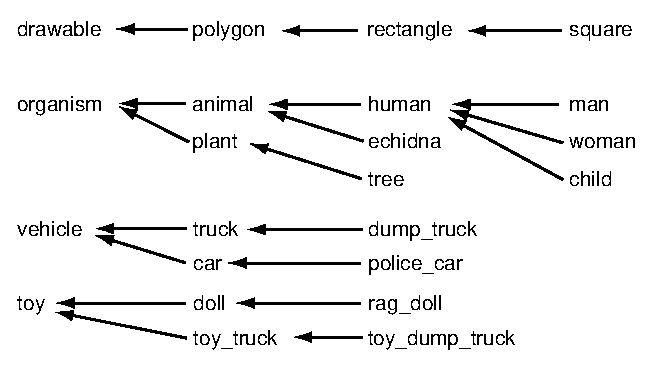
\includegraphics[scale=0.75]{hierarchy}}
\caption{Example inheritance hierarchies.}
\label{figure:inheritance-examples}
\end{figure}

\label{keyword:inherit}
\index{inherit@\lstinline/inherit/}
Concretely, a class inherits from another with the directive
\hbox{\lstinline/inherit $\nt{class-expression}$/},
which effectively includes the entire class $\nt{class-expression}$ within the current one. To
illustrate, let's build a simple model of a part of the animal kingdom.  The following diagram
lists the class hierarchy and methods: every animal eats; a pet is an animal with an owner and a
name; and a pet dog is a pet that barks.

\begin{center}
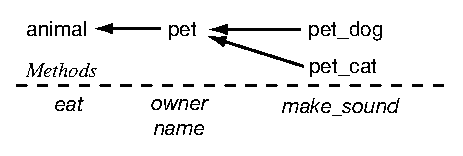
\includegraphics[scale=0.75]{animal1}
\end{center}
%
At the root of the hierarchy is the class \hbox{\lstinline/animal/}, which has a single method \hbox{\lstinline/eat/}.

\begin{ocaml}
# class animal species =
  object
     method eat = Printf.printf "A %s eats.\n" species
  end;;
@
\begin{topoutput}
class animal : string -> object method eat : unit end
\end{topoutput}
@
\end{ocaml}
%
A pet is an animal with an owner and a name.  The class \hbox{\lstinline/pet/} defines
methods \hbox{\lstinline/owner/} and \hbox{\lstinline/name/}, and it also \emph{inherits} from the
class \hbox{\lstinline/animal/}.  The effect of the inheritance is like inclusion, as if the methods of
class \hbox{\lstinline/animal/} were included in the class \hbox{\lstinline/pet/}.

\begin{ocaml}
# class pet ~species ~owner ~name =
  object
     inherit animal species
     method owner : string = owner
     method name  : string = name
  end;;
@
\begin{topoutput}
class pet : species:string -> owner:string -> name:string ->
  object method name : string method owner : string method eat : unit end
\end{topoutput}
@
\end{ocaml}
%
The class \hbox{\lstinline/pet_dog/} is a particular kind of pet that barks.  Once again, the result of the
inheritance is exactly like inclusion.  The class \hbox{\lstinline/pet_dog/} includes the methods of
class \hbox{\lstinline/pet/}, which in turn includes the methods of the class \hbox{\lstinline/animal/}.  The
result is a class that includes all the methods of all the ancestor classes.

\begin{ocaml}
# class pet_dog ~owner ~name =
  object
     inherit pet ~species:"dog" ~owner ~name
     method speak = Printf.printf "%s barks!\n" name
  end;;
@
\begin{topoutput}
class pet_dog : owner:string -> name:string ->
  object
    method speak : unit
    method name : string
    method owner : string
    method eat : unit
  end
\end{topoutput}
@
# let clifford = new pet_dog ~name:"Clifford" ~owner:"Emily";;
@
\begin{topoutput}
val clifford : pet_dog = <obj>
\end{topoutput}
@
# clifford#speak;;
@
\begin{topoutput}
Clifford barks!
\end{topoutput}
@
# clifford#eat;;
@
\begin{topoutput}
A dog eats.
\end{topoutput}
@
\end{ocaml}

\subsection{Method override}

\index{classes!method override}
These previous two examples of inheritance are both forms of specialization where the inheriting
class includes the behavior of the superclass but does not modify it.  It is also possible for a
subclass to modify the behavior by redefining its methods.  For example, since a pet has a name, we
may wish to use the pet's name instead of the species name when it eats.  We can do this by
redefining the method \hbox{\lstinline/eat/}.

\begin{ocaml}
# class pet ~species ~owner ~name =
object
   inherit animal species
   method owner : string = owner
   method name : string = name
   method eat = Printf.printf "%s eats.\n" name
end;;
@
\begin{topoutput}
class pet : species:string -> owner:string -> name:string ->
  object method name : string method owner : string method eat : unit end
\end{topoutput}
@
\end{ocaml}
%
Some dogs are protective about their food.  We can capture this by further
redefining the method \hbox{\lstinline/eat/}.

\begin{ocaml}
# class pet_dog ~owner ~name =
  object (self : 'self)
     inherit pet ~species:"Dog" ~owner ~name as super
     method speak = Printf.printf "%s barks!\n" name
     method prepare_to_eat =
        Printf.printf "%s growls menacingly.\n" name
     method eat =
        self#prepare_to_eat;
        super#eat
  end;;
@
\begin{topoutput}
class pet_dog : ...
\end{topoutput}
@
# let clifford = new pet_dog ~owner:"Emily" ~name:"Clifford";;
@
\begin{topoutput}
val clifford : pet_dog = <obj>
\end{topoutput}
@
# clifford#eat;;
@
\begin{topoutput}
Clifford growls menacingly.
Clifford eats.
\end{topoutput}
@
\end{ocaml}
%
\index{classes!naming a superclass}
The syntax \hbox{\lstinline/inherit $\nt{class-expression}$ as $\nt{identifier}$/} gives a name to the
superclass, which allows the superclass methods to be invoked.  This is useful mainly when the
superclass's methods are overridden in the subclass.  In this case, the method \hbox{\lstinline/eat/} in the
class \hbox{\lstinline/pet_dog/} is a kind of ``wrapper'' method.  It overrides
the \hbox{\lstinline/pet/}'s \hbox{\lstinline/eat/} method by first preparing to eat, then calling the
pet-eat method with the expression \hbox{\lstinline/super#eat/}.

\subsection{Class types}

The design of the inheritance hierarchy can have a major impact on the ease of programming a
system.  This is particularly true for languages based on nominal typing, like C++ or Java, where
subtyping is constrained by the hierarchy.  For example, in a nominal type scheme,
the type of an object corresponds to the class name, so a \hbox{\lstinline/pet_dog/} can be coerced to
a \hbox{\lstinline/pet/}, and then to an \hbox{\lstinline/animal/}, but no other coercions are allowed.

This can be overly restrictive of course.  As the design proceeds we might discover we need new classes.
For the animal example, we might want a class \hbox{\lstinline/farm_animal/}, where animals have owners but
might not have names; or a class \hbox{\lstinline/vocal_animal/} for animals that can vocalize, but might
be wild.  A \hbox{\lstinline/dog/} can be a \hbox{\lstinline/pet/}, a \hbox{\lstinline/farm_animal/}, and also
a \hbox{\lstinline/vocal_animal/}.

In the worst case, the inheritance hierarchy can become complicated because the number of feature
sets is combinatorial.  Languages with interfaces, like Java, try to combat this problem by allowing
a class to satisfy multiple interface definitions.

\begin{java}
interface farm_animal { void eat(); String owner(); };
interface vocal_animal { void eat(); void speak(); }
class dog extends pet implements farm_animal, vocal_animal { $\cdots$ }
\end{java}
%
One drawback of this approach is that the interfaces must be specified at class definition time,
requiring the designer to predict what the useful interfaces will be.

In OCaml, the situation is different.  The inheritance hierarchy constrains the way in which classes
are specified and implemented, but it has no effect on subtyping.  Here is how we could extend the
animal example to support farm animals and vocal animals.

\label{classes:type-inherit}
\begin{ocaml}
# class type farm_animal =
  object
     inherit animal
     method owner : string
  end;;
@
\begin{topoutput}
class type farm_animal = object method owner : string method eat : unit end
\end{topoutput}
@
# class type vocal_animal =
  object
     inherit animal
     method speak : unit
  end;;
@
\begin{topoutput}
class type vocal_animal = object method speak : unit method eat : unit end
\end{topoutput}
@
# (clifford : pet_dog :> farm_animal);;
@
\begin{topoutput}
- : farm_animal = <obj>
\end{topoutput}
@
\end{ocaml}
%
Note that in the \hbox{\lstinline/inherit/} clause, the class type does not take arguments.  In this
context, the name \hbox{\lstinline/animal/} stands for the class type, and the \hbox{\lstinline/inherit/}
directive again acts as textual inclusion.

The main advantage of structural subtyping is that an object can be coerced to any compatible type,
the types do not have to be specified ahead of time.  The disadvantage of course, is that subtyping
may be overly permissive; some coercions might not make sense semantically.

\begin{ocaml}
# class cat ~owner ~name =
  object
     inherit pet ~species:"cat" ~owner ~name
     method speak = Printf.printf "%s meows.\n" name
  end;;
@
\begin{topoutput}
class cat : owner:string -> name:string ->
  object
    method speak : unit
    method name : string
    method owner : string
    method eat : unit
  end
\end{topoutput}
@
# let my_cat = (clifford :> cat);;
@
\begin{topoutput}
val my_cat : cat = <obj>
\end{topoutput}
@
# my_cat#speak;;
@
\begin{topoutput}
Clifford barks!
\end{topoutput}
@
\end{ocaml}

\subsection{Class type constraints and hiding}

\index{classes!type constraints}
\index{classes!hiding}
The type of a class can be constrained with the following syntax, where $\nt{class-type}$ is a class type.

\begin{ocaml}
class $\nt{class-name}$ $\nt{parameter}_1$ $\cdots$ $\nt{parameter}_n$ : $\nt{class-type}$ = $\nt{class-expression}$
\end{ocaml}
%
It is also possible to place constraints on the object type, with an explicit constraint of the form
\hbox{\lstinline/constraint 'self = $\nt{object-type}$/},
or equivalently using the syntax \hbox{\lstinline/$\nt{object-type}$ as 'self/}.

\begin{ocaml}
class cat ~name ~owner =
object (self : 'self)
   constraint 'self = < eat : unit; speak : unit; .. >
   inherit pet ~name ~owner
   method speak = Printf.printf "%s meows.\n" name
end
\end{ocaml}
%
As a programmer, you might want to write a type constraint to ensure that your implementation
matches a specified interface.  However, there are other reasons for using a type constraint.
Unlike the rest of OCaml, type constraints on classes can change how the program behaves.
Here is what you can (and cannot) do with a constraint.

\begin{enumerate}
\item A constraint \emph{cannot} be used hide public methods.
\item A constraint can be used to turn a private method into a public method.
\item A constraint can be used to hide fields and private methods.
\end{enumerate}
%
The restriction on public methods is the same as it is for object types.
If an object has a public method, the method must appear in the type.

\begin{ocaml}
# (object method x = 1 method y = 2 end : < x : int >);;
@
\begin{topoutput}
...
This expression has type < x : int; y : int > but is here used with type
  < x : int >
The second object type has no method y
\end{topoutput}
@
\end{ocaml}
%
The second property, where private methods are made public, may be a little surprising.  It is often
used in cases where a superclass defines a private method that a subclass would like to be made
public.

\begin{ocaml}
# class foo =
  object (self : 'self)
     constraint 'self = < x : int; .. >
     method private x = 1
  end;;
@
\begin{topoutput}
class foo : object method x : int end
\end{topoutput}
@
\end{ocaml}
%
The third kind of constraint, used to hide field and private methods, requires some discussion.
When a class hides a field, or a private method, that field becomes inaccessible to subclasses, and
it also means that the field or method cannot be overridden.  Consider the following class
definitions.

\begin{ocaml}
# class a =
object (self)
   method private f_private = print_string "aaaa\n"
   method test_a = self#f_private
end;;
# class b =
object (self)
   inherit a
   method private f_private = print_string "bbbb\n"
   method test_b =
      self#test_a;
      self#f_private
end;;
# (new b)#test_b;;
@
\begin{topoutput}
bbbb
bbbb
\end{topoutput}
@
\end{ocaml}
%
The method \hbox{\lstinline/f_private/} is private, but it is the same method in both classes.  The definition
of \hbox{\lstinline/f_private/} in class \hbox{\lstinline/b/} \emph{overrides} the definition in class \hbox{\lstinline/a/},
so the result is to print \hbox{\lstinline/bbbb/} twice.
Now let's consider what happens when \hbox{\lstinline/f_private/} is hidden by a type constraint.

\begin{ocaml}
# class type a_type = object method test_a : unit end;;
# class a : a_type =
  object (self)
     method private f_private = print_string "aaaa\n"
     method test_a = self#f_private
  end;;
# class b = $\cdots\hbox{\textit{same as before}}\cdots$;;
# (new b)#test_b;;
@
\begin{topoutput}
aaaa
bbbb
\end{topoutput}
@
\end{ocaml}
%
In this case, the result is different.  By hiding the method \hbox{\lstinline/f_private/} in
class \hbox{\lstinline/a/}, it can't be used or overridden in subclass \hbox{\lstinline/b/}, and the behavior of
the program is changed.

The property is the same for fields.  When a field is hidden y a type constraint, it is no longer
accessible to subclasses.  New field definitions with the same name in subclasses are independent.
  
\subsection{Classes and class types as object types}

As we have mentioned, a class is not a type, but the class name stands for an object type
when used in the context of a type expression.  The same holds for class types---a class type is the
type of a class, but it also stands for the type of an object when used in context of a type
expression.  The object type is formed from a class type by omitting the field types.
The following table lists some examples of equivalent types.

\begin{center}
\begin{tabular}{lll}
Class type & Object type & Simplified\\
\hline
\begin{minipage}[t]{1.5in}
\begin{ocamllisting}
class type t1 =
object
   val x : int
   method y : int
end
\end{ocamllisting}
\end{minipage}
&
\begin{minipage}[t]{1.5in}
\begin{ocamllisting}
type t1 = < y : int >
\end{ocamllisting}
\end{minipage}
\\
\begin{minipage}[t]{1.5in}
\begin{ocamllisting}
class type t2a =
object ('self)
   val x : int
   method f1 : t2a
   method f2 : 'self  
end

class type t2b =
object ('self)
   inherit t2a
   method f3 : unit
end
\end{ocamllisting}
\end{minipage}
&
\begin{minipage}[t]{1.5in}
\begin{ocamllisting}
type t2a =
   < f1 : t2a;
     f2 : 'self
    > as 'self



type t2b =
   < f1 : t2a;
     f2 : 'self;
     f3 : unit
   > as 'self
\end{ocamllisting}
\end{minipage}
&
\begin{minipage}[t]{1in}
\begin{ocamllisting}
type t2a =
   < f1 : t2a;
     f2 : t2a
    >



type t2b =
   < f1 : t2a;
     f2 : t2b;
     f3 : unit
   >
\end{ocamllisting}
\end{minipage}
\end{tabular}
\end{center}
%
The role of \hbox{\lstinline/'self/} in these types is subtle and important.  In class
type \hbox{\lstinline/t2a/}, the method \hbox{\lstinline/f1/} returns an object of type \hbox{\lstinline/t2a/}, which
means that it is an object with exactly two methods, \hbox{\lstinline/f1/} and \hbox{\lstinline/f2/}.  The
method \hbox{\lstinline/f2/} returns an object of the same type as \hbox{\lstinline/self/}---which,
for an object of type \hbox{\lstinline/t2a/}, has the same methods \hbox{\lstinline/f1/} and \hbox{\lstinline/f2/}.

However, when the subclass \hbox{\lstinline/t2b/} is formed, a new method \hbox{\lstinline/f3/} is added.  The
method \hbox{\lstinline/f1/} returns an object of type \hbox{\lstinline/t2a/}, having two methods \hbox{\lstinline/f1/}
and \hbox{\lstinline/f2/}; but the method \hbox{\lstinline/f2/} returns an object of type \hbox{\lstinline/'self/},
now having three methods \hbox{\lstinline/f1/}, \hbox{\lstinline/f2/}, and \hbox{\lstinline/f3/}.

\label{keyword:hash-class}
\index{classes!\#types@\lstinline/#/types}
\index{\#!class types}
There are actually two kinds of object types that are formed from class names: exact and open types.
The type expression $\nt{class-name}$ stands for the type of objects having exactly the
methods of the class $\nt{class-name}$ and the type expression \hbox{\lstinline/#$\nt{class-name}$/}
stands for objects having those methods, and possibly more.  In other words, a type expression
\hbox{\lstinline/#$\nt{class-name}$/} stands for an open object type.

\begin{center}
\begin{tabular}{ll}
Type expression & Object type\\
\hline
\begin{minipage}[t]{2in}
\begin{ocamllisting}
t1
#t1
\end{ocamllisting}
\end{minipage}
&
\begin{minipage}[t]{2in}
\begin{ocamllisting}
< y : int >
< y : int; .. >
\end{ocamllisting}
\end{minipage}
\\
\begin{minipage}[t]{2in}
\begin{ocamllisting}
t2a
#t2a
\end{ocamllisting}
\end{minipage}
&
\begin{minipage}[t]{2in}
\begin{ocamllisting}
< f1 : t2a; f2 : 'self > as 'self
< f1 : t2a; f2 : 'self; .. > as 'self
\end{ocamllisting}
\end{minipage}
\\
\begin{minipage}[t]{2in}
\begin{ocamllisting}
#t2b
\end{ocamllisting}
\end{minipage}
&
\begin{minipage}[t]{2in}
\begin{ocamllisting}
< f1 : t2a;
  f2 : 'self;
  f3 : unit;
  .. > as 'self
\end{ocamllisting}
\end{minipage}
\end{tabular}
\end{center}
%
Just like an open object type, a type expression \hbox{\lstinline/#$\nt{class-name}$/} is polymorphic.

\begin{ocaml}
# type s2a = #t2a;;
@
\begin{toperror}
Characters 4-15:
  type s2a = #t2a;;
      ^^^^^^^^^^^
A type variable is unbound in this type declaration.
In definition #t2a as 'a the variable 'a is unbound
\end{toperror}
@
# type 'a s2a = #t2a as 'a;;
@
\begin{topoutput}
type 'a s2a = 'a constraint 'a = #t2a
\end{topoutput}
@
\end{ocaml}

\section{Inheritance is not subtyping}

\index{classes!inheritance \emph{vs}. subtyping}
Let's summarize the operations that can be performed through inheritance.
One may:
%
\begin{itemize}
\item add new fields and new private methods,
\item add new public methods,
\item override fields or methods, but the type can't be changed.
\end{itemize}
%
Fields and private methods don't appear in the object type, and method override isn't allowed to
change the method's type.  So from a typing perspective, if a class $B$ is a subclass of $A$, it
might have more methods than $A$, but everything else is unchanged.  By width subtyping
(Section~\ref{section:width-subtyping}), this will usually mean that the object type for $B$ is a
subtype of the object type for $A$.  In fact, in many languages, subclassing and subtyping are the
same, and it isn't possible to have one without the other.

Unfortunately, the correspondence is sound only in the case where the object type is covariant
in \hbox{\lstinline/'self/}; in other words, when the object has no binary methods.  Consider a class
type \hbox{\lstinline/comparable/} for objects that can be compared.
\label{page:comparable}

\begin{ocaml}
(* less-than: negative; equal: zero; greater-than: positive *)
type comparison = int

class type comparable =
object ('self)
   method compare : 'self -> comparison
end
\end{ocaml}
%
The method \hbox{\lstinline/compare/} is a binary method; it takes another object of type \hbox{\lstinline/'self/}
and performs a comparison.  The implementations use the usual technique of adding a
method \hbox{\lstinline/representation/} to expose the internal representation so that the comparison can
be implemented.\footnote{Note that subtraction can only be used to compare small
integers.}

\begin{ocaml}
class int_comparable (i : int) =     class string_comparable (s : string) =
object                               object
   method representation = i            method representation = s
   method compare (j : 'self) =         method compare (s2 : 'self) =
      i - j#representation                 String.compare s s2#representation
end                                  end
\end{ocaml}
%
We might later decide to implement some subclasses for printable, comparable objects.
%
\begin{ocaml}
class int_print_comparable i =       class string_print_comparable s =
object (_ : 'self)                   object (_ : 'self)
   inherit int_comparable i             inherit string_comparable s
   method print = print_int i           method print = print_string s
end                                  end
\end{ocaml}
%
We might expect that a printable and comparable integer is also a comparable integer.  However, the
expected coercions fail.

\begin{ocaml}
# (new int_comparable 1 :> comparable);;
@
\begin{topoutput}
... This expression cannot be coerced ...
\end{topoutput}
@
# (new int_print_comparable 1 :> int_comparable);;
@
\begin{topoutput}
... This expression cannot be coerced ...
\end{topoutput}
@
\end{ocaml}
%
For an intuitive explanation, consider what would happen if the subtype relation
\hbox{\lstinline/int_comparable $\subtype$ comparable/} held.
The relation \hbox{\lstinline/string_comparable $\subtype$ comparable/} would hold as well, allowing us to
perform an unsound comparison of strings and integers.

\begin{ocaml}
(* !!FAKE--THESE OPERATIONS ARE UNSOUND!! *)
# let i = (new int_comparable 1 :> comparable);;
@
\begin{topoutput}
i : comparable = < obj >
\end{topoutput}
@
# let s = (new string_comparable "Hello" :> comparable);;
@
\begin{topoutput}
s : comparable = < obj >
\end{topoutput}
@
# i#compare s;;
@
\begin{topoutput}
???
\end{topoutput}
@
\end{ocaml}
%
The real problem is the the method \hbox{\lstinline/compare/} is \emph{contravariant} in the
type \hbox{\lstinline/'self/} because it takes a value of type \hbox{\lstinline/'self/} as an argument.  This is
the opposite of what it normally is.  Here are the object types that correspond to the classes and
class types.

\begin{ocaml}
comparable = < compare : 'self -> bool > as 'self
int_comparable =
   < representation : int;
     compare : 'self -> bool > as 'self
int_print_comparable =
   < representation : int;
     compare : 'self -> bool;
     print : unit > as 'self
\end{ocaml}
%
Let's try to carry out a proof of the subtyping relation
\hbox{\lstinline/int_comparable $\subtype$ comparable/}
to see where it goes wrong.  The type \hbox{\lstinline/'self/} in each case corresponds
to the type name, so we are try to show the following.

\begin{ocaml}
< representation : int; compare : int_comparable -> bool >
$\subtype$ < compare : comparable -> bool >
\end{ocaml}
%
Attempted proof:
\begin{itemize}
\item 
The types are recursive, so we first assume that subtyping holds on the type
names \hbox{\lstinline/int_comparable $\subtype$ comparable/}.
\item
By width subtyping, the method \hbox{\lstinline/representation/} can be dropped.
Show:
\begin{ocaml}
< compare : int_comparable -> bool > $\subtype$ < compare : comparable -> bool >
\end{ocaml}
\item
By depth subtyping, show:
\begin{ocaml}
(int_comparable -> bool) $\subtype$ (comparable -> bool)
\end{ocaml}
\item
By function subtyping, show:
\begin{ocaml}
comparable $\subtype$ int_comparable
\end{ocaml}
\item This is the opposite of the assumption, so the proof fails.
\end{itemize}

% \subsubsection{Generic functions and binary methods}

Of course, this doesn't mean that we can't write generic functions of comparable objects, it simply
means that the functions should use the open type \hbox{\lstinline/#comparable/}, not the exact
non-polymorphic type \hbox{\lstinline/comparable/}.

\begin{ocaml}
# let sort (l : #comparable list) = List.sort (fun e1 e2 -> e1#compare e2) l;;
@
\begin{topoutput}
val sort : (#comparable as 'a) list -> 'a list = <fun>
\end{topoutput}
@
# let l = List.map (new int_print_comparable) [9; 1; 6; 4];;
@
\begin{topoutput}
val l : int_print_comparable list = [<obj>; <obj>; <obj>; <obj>]
\end{topoutput}
@
# List.iter (fun i -> i#print) (sort l);;
@
\begin{topoutput}
1469
\end{topoutput}
@
\end{ocaml}

% \subsubsection{Bounded methods}

We might be willing to accept the fact that there are no useful objects with exact
type \hbox{\lstinline/comparable/}, but what about the relation between the
types \hbox{\lstinline/int_print_comparable/} and \hbox{\lstinline/int_comparable/}?  If it seems that the
subtyping relation should hold, the solution is to avoid the use of binary methods.  The
method \hbox{\lstinline/compare/} doesn't really need an argument of type \hbox{\lstinline/'self/},
it just needs an object with the same representation.  The classes can be reimplemented
to use a constrained argument type.

\begin{ocaml}
class int_comparable (i : int) =
object
   method representation = i
   method compare : 'a. (< representation : int; .. > as 'a) -> comparison =
      (fun j -> Pervasives.compare i j#representation)
end

class int_print_comparable i =
object
   inherit int_comparable i
   method print = print_int i
end
\end{ocaml}
%
It now holds that \hbox{\lstinline/int_print_comparable/} is a subtype of \hbox{\lstinline/int_comparable/}, but
there are several drawbacks.  One is that the new objects no longer have
type \hbox{\lstinline/#comparable/}, so it isn't possible to write truly generic functions.  Another
problem is that the types get quickly complicated.  Still, with some effort, we get what we want.

\begin{ocaml}
# let compare_int (e1 : #int_comparable) (e2 : #int_comparable) =
     e1#compare e2;;
@
\begin{topoutput}
val compare_int : #int_comparable -> #int_comparable -> comparison = <fun>
\end{topoutput}
@
# let sort_int (l : #int_comparable list) =
     List.sort compare_int l;;
@
\begin{topoutput}
val sort_int : (#int_comparable as 'a) list -> 'a list = <fun>
\end{topoutput}
@
# let l = List.map (new int_print_comparable) [9; 1; 3; 2];;
@
\begin{topoutput}
val l : int_print_comparable list = [<obj>; <obj>; <obj>; <obj>]
\end{topoutput}
@
# List.iter (fun i -> i#print) (sort_int l);;
@
\begin{topoutput}
1239
\end{topoutput}
@
\end{ocaml}

\labelsection{modules-classes}{Modules and classes}

OCaml includes two major systems for modularity and abstraction: the module system and the object
system.  In many respects, the two systems are quite similar.  Both provide mechanisms for
abstraction and encapsulation, for subtyping (by omitting methods in objects, and omitting fields in
modules), and for inheritance (objects use \hbox{\lstinline/inherit/}; modules use \hbox{\lstinline/include/},
Section~\ref{section:include}).  However, the two systems are not comparable.  On the one hand,
objects have an advantage: objects are first-class values, and modules are not---in other words,
modules do not support dynamic lookup.  On the other hand, modules have an advantage: modules
can contain type definitions, and objects cannot.

We have already suggested that modules are handy for hiding internal representations in the definition of
binary methods.  For example, let's use the module to hide the representation of a comparable object.

\begin{ocaml}
module type IntComparableSig =
sig
   type rep

   class int_comparable : int ->
   object ('self)
      method representation : rep
      method compare : 'self -> comparison
   end
end

module IntComparable : IntComparableSig =
struct
   type rep = int

   class int_comparable (i : int) =
   object (_ : 'self)
      method representation = i
      method compare (j : 'self) =
         Pervasives.compare i j#representation
   end
end
\end{ocaml}
%
This method of hiding the representation also has the side-effect that it is no longer possible to
construct an object of type \hbox{\lstinline/int_comparable/} without using the
class \hbox{\lstinline/int_comparable/}.  We can use this to our advantage.  In the animal example, if we
wish to ensure that dogs cannot be turned into cats, we can give the cats a ``certificate'' that
``justifies'' their authenticity.

\begin{ocaml}
module type CatSig =
sig
   type cert

   class cat : owner:string -> name:string ->
   object
      inherit pet
      method cert : cert
      method speak : unit
   end
end

module Cat : CatSig =
struct
   type cert = unit

   class cat ~owner ~name =
   object
       inherit pet ~species:"cat" ~owner ~name
       method cert = ()
       method speak = Printf.printf "%s meows.\n" name
   end
end
\end{ocaml}
%
\index{cat certificates}
It doesn't matter what the certificate is, just that it is abstract.  Of course, this technique
mainly prevents accidental coercions.  If a dog really wants to become a cat, it can take the
certificate from one of them.

Functors can also be useful in class construction.  For example, there are many specific kinds of
comparable objects, integers, floating-point values, strings, pairs of \hbox{\lstinline/comparable/}
objects, \emph{etc}.  All we need to build one of these is a function to compare the values.
The generic class is described the usual way.

\begin{ocaml}
(* less-than: negative; equal: zero; greater-than: positive *)
type comparison = int

class type comparable =
object ('self)
   method compare : 'self -> comparison
end;;
\end{ocaml}
%
To build a specific kind of comparable items, we need a function to compare the values.  We can build
a generic module as a functor that takes the type of items and the comparison as an argument, and produces
a new class of comparable items.

\begin{ocaml}
module type CompareSig =
sig
   type t
   val compare : t -> t -> comparison
end;;

module type ComparableSig =
sig
   type t
   type rep

   class element : t ->
   object ('self)
       method representation : rep
       method compare : 'self -> comparison
   end
end;;

module MakeComparable (Compare : CompareSig)
: ComparableSig with type t = Compare.t =
struct
   type t = Compare.t
   type rep = Compare.t

   class element (x : t) =
   object (self : 'self)
      method representation = x
      method compare (item : 'self) =
         Compare.compare x item#representation
   end
end;;
\end{ocaml}
%
The representation type \hbox{\lstinline/rep/} is abstract, but the type of element values \hbox{\lstinline/t/} is
not.  The method \hbox{\lstinline/compare/} simply uses the provided function \hbox{\lstinline/Compare.compare/}
to compare the representations.

\labelsection{poly-methods}{Polymorphic methods and virtual classes}

Let's turn to another example of object-oriented programming, this time more computational.
A \emph{collection}, in general, is like a set of elements.  There are many kinds of collections,
some based on implementations like arrays or lists, and others based on access patterns, like stacks
and queues.  Figure~\ref{figure:collection-hierarchy} shows a partial inheritance hierarchy.

\begin{figure}
\centerline{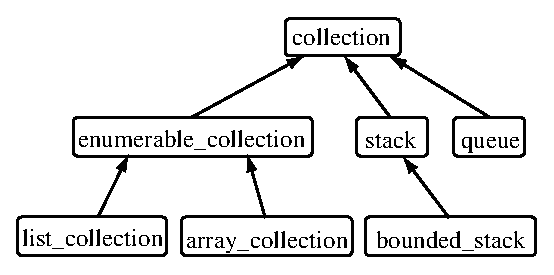
\includegraphics[scale=0.75]{collection}}
\caption{Hierarchy of collections}
\label{figure:collection-hierarchy}
\end{figure}

It won't matter much what the elements are, so for now we'll just assume the elements can be
printed.  It might also be useful to build polymorphic collections, but we'll leave that topic for
the Chapter~\ref{chapter:polyclasses}.

\begin{ocaml}
class type element = object method print : unit end
\end{ocaml}
%
At the root of the inheritance hierarchy is the type \hbox{\lstinline/collection/}, which represents the
features that all collections have in common.  What are those features?  It can't be implementation
or access pattern, because those features change for different kinds of collections.  In fact, the
type \hbox{\lstinline/collection/} by itself is pretty useless.  We'll assume it has a
method \hbox{\lstinline/length/} that returns the number of elements in the collection.

\begin{ocaml}
class type collection =
object
   method length : int
end
\end{ocaml}
%
At the middle of the hierarchy is the ``\hbox{\lstinline/enumerable_collection/},'' which represents
collections where the elements can be enumerated, using functions like \hbox{\lstinline/iter/} to iterate
over all the elements, or \hbox{\lstinline/fold/} to compute a value from all the elements.  The method types
correspond to the function types in the standard libraries \hbox{\lstinline/List/}
and \hbox{\lstinline/Array/}.  We still haven't implemented a concrete collection, so this is still a class
type.

\begin{ocaml}
class type enumerable_collection =
object
   inherit collection
   method iter : (element -> unit) -> unit
   method fold : ('a -> element -> 'a) -> 'a -> 'a
end;;
\end{ocaml}

\subsection{Polymorphic methods}

\index{classes!polymorphic methods}
Next, \hbox{\lstinline/list/} and \hbox{\lstinline/array/} are two concrete
kinds of collections that differ mainly in how they are accessed; a \hbox{\lstinline/list/} is a stack,
while an \hbox{\lstinline/array/} allows random access.  However, when we try to provide a concrete list
implementation, we encounter an error because the method \hbox{\lstinline/fold/} is polymorphic.

\begin{ocaml}
# class broken_list_collection =
  object
     $\cdots$
     method fold f x = List.fold_left f x elements
  end;;
@
\begin{toperror}
Characters 5-328: ...
Some type variables are unbound in this type:
...
The method fold has type ('a -> element -> 'a) -> 'a -> 'a where 'a
is unbound
\end{toperror}
@
\end{ocaml}
%
\label{types:polymorphic-methods}
The problem here is that OCaml assumes that
the \emph{class} must be polymorphic, not the \emph{method} (which is what we intend).  OCaml allows
methods to be polymorphic, but they must be annotated explicitly using the following syntax.

\begin{ocaml}
method $\nt{identifier}$ : '$\nt{type-variable}$ $\cdots$ '$\nt{type-variable}$. $\nt{type}$ = $\nt{expression}$
\end{ocaml}
%
\label{classes:type-quantifier}
The type expression \hbox{\lstinline/'$\nt{type-variable}$ $\cdots$ '$\nt{type-variable}$. $\nt{type}$/} is
called a \emph{universally quantified type}, and the type variables before the \hbox{\lstinline/./} are
bound specifically in the method type $\nt{type}$, not for the class as a whole.  Note that the type
constraint is required to occur right after the method name, so functions must be written explicitly.
Here is a corrected definition, which is now accepted by the top-loop.  Note that in the class type,
the type variable is not required.

\begin{ocaml}
# class list_collection =
  object
     val mutable elements : element list = []
     method length = List.length elements

     method add x = elements <- x :: elements
     method remove = elements <- List.tl elements

     method iter f = List.iter f elements
     method fold : 'a. ('a -> element -> 'a) -> 'a -> 'a =
        (fun f x -> List.fold_left f x elements)
  end;;
@
\begin{topoutput}
class list_collection :
object
   ...
   method fold : ('a -> element -> 'a) -> 'a -> 'a
end
\end{topoutput}
@
\end{ocaml}
%
Continuing with our example, the \hbox{\lstinline/array_collection/} has a similar definition.  Some
differences are that the size of the array is determined at instantiation time, and
the \hbox{\lstinline/Array/} module doesn't provide a \hbox{\lstinline/fold/} function, so we have to code it
manually.

\begin{ocaml}
class array_collection size init =
object
   val elements = Array.create size init
   method length = size
   method set i x = elements.(i) <- x
   method get i = elements.(i)
   method iter f = Array.iter f elements
   method fold : 'a. ('a -> element -> 'a) -> 'a -> 'a =
      (fun f x ->
         let rec loop i x =
            if i = size then x else loop (i + 1) (f x elements.(i))
         in
         loop 0 x)
end;;
\end{ocaml}

\subsection{Virtual (abstract) classes and methods}

\index{classes!virtual}
At this point, we have two class types, \hbox{\lstinline/collection/}
and \hbox{\lstinline/enumerable_collection/}; and two concrete classes, \hbox{\lstinline/list_collection/}
and \hbox{\lstinline/array_collection/}.  The reason for using class types for the former is because there
are no actual instances of \hbox{\lstinline/collection/} or \hbox{\lstinline/enumerable_collection/}; the only
actual instances are of the subclasses.

Now, suppose we wanted to be able to print a collection.  We could implement a
method \hbox{\lstinline/print/} for each of the concrete classes \hbox{\lstinline/list/} and \hbox{\lstinline/array/},
but in fact the implementations can be written the same way.

\begin{ocaml}
   method print = self#iter (fun element -> element#print)
\end{ocaml}
%
A better way to implement it is to ``lift'' the implementation into the \hbox{\lstinline/enumerable_collection/}
superclass.  The problem is that \hbox{\lstinline/enumerable_collection/} is a class type, not a class, so
it can't contain code.

The solution is to define \hbox{\lstinline/enumerable_collection/} as a \emph{virtual class}, which is a
class where some or all of the method implementations are omitted.  In our example, the
methods \hbox{\lstinline/iter/} and \hbox{\lstinline/fold/} are to be implemented in subclasses, so they are
omitted, but the method \hbox{\lstinline/print/} can be implemented.  A method where the implementation is
omitted is called a \emph{virtual method}, and it is declared with the syntax

\index{virtual@\lstinline/virtual/}
\label{keyword:virtual}
\begin{ocaml}
method virtual $\nt{identifier}$ : $\nt{type}$.
\end{ocaml}
%
Any class that contains a virtual method must also be declared virtual, with the
syntax \hbox{\lstinline/class virtual/}.  For completeness in our example, we also declare the
class \hbox{\lstinline/collection/} as virtual, so that it can be inherited by the \hbox{\lstinline/collection/}
class.

\begin{ocaml}
class virtual collection =
object
   method virtual length : int
end;;

class virtual enumerable_collection =
object (self : 'self)
   inherit collection
   method virtual iter : (element -> unit) -> unit
   method virtual fold : 'a. ('a -> element -> 'a) -> 'a -> 'a
   method print = self#iter (fun element -> element#print)
end;;
\end{ocaml}
%
Virtual classes cannot be instantiated.  However, once the methods have been implemented (by a
subclass), the virtual status of a class can be removed.

\begin{ocaml}
# class list_collection =
  object
     inherit enumerable_collection

     val mutable elements : element list = []
     method length = List.length elements
     method add x = elements <- x :: elements
     method remove = elements <- List.tl elements
     method iter f = List.iter f elements
     method fold : 'a. ('a -> element -> 'a) -> 'a -> 'a =
        (fun f x -> List.fold_left f x elements)
  end;;
@
\begin{topoutput}
class list_collection :
  object
    val mutable elements : element list
    method add : element -> unit
    method fold : ('a -> element -> 'a) -> 'a -> 'a
    method iter : (element -> unit) -> unit
    method length : int
    method print : unit
    method remove : unit
  end
\end{topoutput}
@
\end{ocaml}

\subsection{Terminology}

\index{classes!virtual \emph{vs}. abstract}
Classes with omitted implementations are a standard feature of many object-oriented languages.  In
mainstream terminology, they are called \emph{abstract} classes, and a ``virtual method'' is a
method that is resolved using dynamic lookup (as opposed to a ``static method'' that uses static lookup).

The non-standard terminology OCaml uses can be quite confusing, especially to those not familiar
with OCaml, or those just learning the language.  However, there is a good argument that OCaml uses
the correct terms, and mainstream terminology is inaccurate.  Here are selected definitions of the terms
``abstract'' and ``virtual,'' taken from the American-Heritage dictionary of the English
Language~\cite{american-heritage-2000}.

\begin{description}
\item[\textbf{ab$\cdot$stract}]

$\ldots$ 4.{} Thought of or stated without reference to a specific instance $\ldots$

\item[\misspelled{\textbf{vir$\cdot$tu$\cdot$al}}]

1.{} Existing or resulting in essence or effect though not in actual fact, form, or name$\ldots$
\end{description}
%
Put more loosely, if something is abstract, it means it exists but it is not entirely specified or
defined; if something is virtual, it appears to exist, but doesn't in actual fact.  In this sense,
virtual is the more appropriate term, because a virtual class can be used in all ways like a normal
class---except for one: it can't be instantiated because it doesn't fully exist.

\subsection{Stacks}

Returning to our example, let's move back up the hierarchy, and consider the \hbox{\lstinline/stack/}
class.  Stacks are defined by their behavior: elements are pushed onto the top of the stack, and
taken from the top of the stack, in last-in-first-out (LIFO) order.  A generic stack is a virtual
class with two virtual methods: \hbox{\lstinline/push : element -> unit/} pushes an element onto the top of
the stack, and \hbox{\lstinline/pop : element/} removes and returns the top element.  In addition, we
include two derived methods: \hbox{\lstinline/dup : unit/} duplicates to topmost element of the stack,
and \hbox{\lstinline/swap : unit/} swaps the top two elements.

\begin{ocaml}
class virtual stack =
object (self : 'self)
   inherit collection
   method virtual push : element -> unit
   method virtual pop  : element
   method dup =
      let x = self#pop in
      self#push x;
      self#push x
   method swap =
      let x1 = self#pop in
      let x2 = self#pop in
      self#push x1;
      self#push x2
end;;
\end{ocaml}
%
Let's implement a real subclass \hbox{\lstinline/bounded_stack/} in terms of arrays.
The \hbox{\lstinline/bounded_stack/} inherits from the virtual class \hbox{\lstinline/stack/}, and implements the
methods \hbox{\lstinline/push/} and \hbox{\lstinline/pop/} in terms of array operations.

\begin{ocaml}
class bounded_stack size =
let dummy = object method print = () end in
object
   inherit stack

   val data = new array_collection size dummy
   val mutable index = 0

   method push x =
      if index = size then
         raise (Failure "stack is full");
      data#set index x;
      index <- index + 1
   method pop =
      if index = 0 then
         raise (Failure "stack is empty");
      index <- index - 1;
      data#get index
   method length = data#length
end;;
\end{ocaml}
%
The class \hbox{\lstinline/bounded_stack/} stores its values in an array, initialized to a dummy value.
The method \hbox{\lstinline/push/} adds an element if there is room, and the method \hbox{\lstinline/pop/} returns
an element if the stack is nonempty.  The methods \hbox{\lstinline/dup/} and \hbox{\lstinline/swap/} are
implemented by the superclass \hbox{\lstinline/stack/}.

\subsection{Lists and stacks}

The class \hbox{\lstinline/bounded_stack/} demonstrates two relationships: it \emph{is-a} stack, so it
inherits from the class \hbox{\lstinline/stack/}; and it \emph{has-a} array, which it includes as a field
that it uses to implement the virtual methods needed to implement a \hbox{\lstinline/stack/}.

Another way to build a stack is in terms of a list, but in this case the stack and list are so
similar, we might want to say that a stack \emph{is-a} list, and inherit from the
class \hbox{\lstinline/list_collection/} directly.  OCaml supports multiple inheritance; we
simply \hbox{\lstinline/inherit/} from each superclass.

\begin{ocaml}
# class unbounded_stack =
  object (self : 'self)
     inherit list_collection
     inherit stack

     method push x = self#add x
     method pop =
        let x = self#head in
        self#remove;
        x
  end;;
@
\begin{topoutput}
class unbounded_stack :
  object
    val mutable elements : element list
    method add : element -> unit
    method dup : unit
    method fold : ('a -> element -> 'a) -> 'a -> 'a
    ...
  end
\end{topoutput}
@
\end{ocaml}
%
The resulting class has the methods and fields of both superclasses, so in addition to being a
stack, it is also an \hbox{\lstinline/enumerable_collection/} (and a \hbox{\lstinline/list_collection/}).

Is this construction appropriate?  It depends on whether it is acceptable to view the stack as a
list.  For example, the class \hbox{\lstinline/unbounded_stack/} has two methods to add an element to the
stack: \hbox{\lstinline/push/} and \hbox{\lstinline/add/}, and they are the same (\hbox{\lstinline/push/}
calls \hbox{\lstinline/add/}).  If it is acceptable for subclasses to override one of the methods and not
the other, then the multiple inheritance is acceptable; otherwise it is not.  Certainly, it is not
appropriate for the \hbox{\lstinline/bounded_collection/} to inherit from the \hbox{\lstinline/array_collection/}
because the array's unrestricted \hbox{\lstinline/set/} and \hbox{\lstinline/get/} operations are not appropriate
for a stack.  We'll see more about multiple inheritance in the next chapter.

% -*-
% Local Variables:
% Mode: LaTeX
% fill-column: 100
% TeX-master: "paper"
% TeX-command-default: "LaTeX/dvips Interactive"
% End:
% -*-
% vim:tw=100:fo=tcq:
